\section{Conjugate Gradient Iteration}
\label{sec:2}

\subsection{Krylov methods and the minimization property}
\label{sec:2.1}

\begin{defi}
  Given a nonsingular $A\in\mathbb{C}^{N\times N}$ and $y\neq
  \mathbf{0}\in\mathbb{C}^N$, the $n$th \emph{Krylov subspace}
  $\mathcal{K}_n(A,y)$ generated by $A$ from $y$ is
  $$\mathcal{K}_n:=\mathcal{K}_n(A,y)=\text{\textbf{span}}(y,Ay,\ldots,A^{n-1}y).$$
\end{defi}

\begin{defi}
  A \emph{Krylov space method} for solving a linear system $Ax=b$ is
  an iterative method starting from some initial approximation $x_0$,
  the corresponding residual $r_0:=b-Ax_0$ and generating for
  all or at least most $n$, until it possibly finds the exact
  solution, iterates $x_n$ such that
  $$x_n-x_0=q_{n-1}(A)r_0\in \mathcal{K}_n(A,r_0)$$
  with a polynomial $q_{n-1}$ of exact degree $n-1$. For some $n$,
  $x_n$ may not exist or $q_{n-1}$ may have lower degree. 
\end{defi}

\begin{exm}
  The two such methods that we will discuss in depth, conjugate
  gradient and GMRES, minimize, at the $k$th iteration, some measure
  of error over the affine space $$x_0+\mathcal{K}_k,$$
  where $x_0$ is the initial iterate and the $k$th Krylov subspace
  $\mathcal{K}_k$
  is $$\mathcal{K}_k=\mathcal{K}_k(A,r_0)=\text{\textbf{span}}(r_0,Ar_0,
  \ldots,A^{k-1}r_0)$$
  for $k\geq 1.$
\end{exm}

\begin{rmk}
  Unlike the classical work, in the following sections, we will begin
  with a description of what the algorithm does and the consequences
  of the minimization property of the iterates. After that we describe
  termination criterion, performance, preconditioning, and at the very
  end, the implementation.
\end{rmk}


\begin{defi}
  A linear system $Ax=b$ is called \emph{symmetric positive
    definite (spd)} systems if A is symmetric and positive definite,
  i.e., $$A=A^T\ \text{and } x^TAx>0\ \text{for all } x\neq 0$$
  CG iteration is intended to solve symmetric positive definite (spd) systems.
\end{defi}

\begin{defi}
  Given a symmetric positive definite matrix $A$, we may define a norm
  by
  \begin{equation}
    \label{eq:2.1}
    \|x\|_{A}=\sqrt{x^TAx}
  \end{equation}
  which is called the $A$-norm.
\end{defi}



\begin{lemma}
  The $k$th iterate $x_k$ of CG minimizes
  \begin{equation}
    \label{eq:2.2}
    \phi(x)=\frac{1}{2}x^TAx - x^Tb
  \end{equation}
  over $x_0+\mathcal{K}_k$. If $\phi(\tilde{x})$ is the minimal value
  in $\mathbb{R}^N$, then $\tilde{x}=x^*:=A^{-1}b$.
\end{lemma} 

\begin{proof}
  $\phi(\tilde{x})$ is the minimal value, then
  \begin{equation*}
    \nabla\phi(\tilde{x})=A\tilde{x}-b = 0.\qedhere
  \end{equation*}
\end{proof}

\begin{lemma}[minimization property of CG iteration]
  Let $\mathcal{S}\subset \mathbb{R}^N$. If $x_k$ minimizes $\phi$
  over $\mathcal{S}$ then $x_k$ also minimizes
  $\|x^*-x\|_A=\|r\|_{A^{-1}}$ over $\mathcal{S}$.
\end{lemma}

\begin{proof}
  Note that
  $$\|x-x^*\|^2_A = x^TAx - x^TAx^*
  -(x^*)^TAx+(x^*)^TAx^*.$$
  Since $A$ is symmetric and $Ax^*=b$,
  $$-x^TAx^*-(x^*)^TAx = -2x^TAx^*=-2x^Tb.$$
  Therefore $$\|x-x^*\|_A^2=2\phi(x)+(x^*)^TAx^*.$$
  Since $(x^*)^TAx^*$ is independent of $x$, minimizing $\phi$ is
  equivalent to minimizing $\|x-x^*\|_A^2$ and hence to minimizing
  $\|x-x^*\|_A.$

  If $e=x-x^*$ then
  $$\|e\|^2_A=e^TAe=(A(x-x^*))^TA^{-1}(A(x-x^*))=\|b-Ax\|_{A^{-1}}^2$$
  and hence the $A$-norm of the error is also $A^{-1}$-norm of the residual.
\end{proof}

\begin{rmk}
  We will use this lemma in the particular case that
  $\mathcal{S}=x_0+\mathcal{K}_k$ for some k.
\end{rmk}

\subsection{Consequences of the minimization property}
\label{sec:2.2}

\begin{lemma}
  In the $k$th step of CG iteration, we have
  \begin{equation}
    \label{eq:2.4}
    \|x^*-x_k\|_A=\min_{p\in\mathbf{P}_k,p(0)=1}\|p(A)(x^*-x_0)\|_A
  \end{equation}
  where $\mathbf{P}_k$ denotes the set of polynomials of degree $k$.
\end{lemma}

\begin{proof}
  Lemma 1.2.7 implies that since $x_k$ minimizes $\phi$ over
  $x_0+\mathcal{K}_k$
  \begin{equation}
    \label{eq:2.3}
    \|x^*-x_k\|_A\leq\|x^*-\omega\|_A
  \end{equation}
  for all $\omega\in x_0+\mathcal{K}_k$ can be written as
  $$\omega = \sum\limits_{j=0}^{k-1}\gamma_jA^jr_0+x_0$$
  for some coefficients $\{\gamma_j\}$, we can express $x^*-\omega$ as
  $$x^*-\omega=x^*-x_0-\sum\limits_{j=0}^{k-1}\gamma_jA^jr_0.$$
  Since $Ax^*=b$ we have $$r_0=b-Ax_0=A(x^*-x_0)$$ and therefore
  $$x^*-\omega=x^*-x_0-\sum\limits_{j=0}^{k-1}\gamma_jA^{j+1}(x^*-x_0)=p(A)(x^*-x_0)$$
  where the polynomial $p(z)$ has degree $k$ and satisfies
  $p(0)=1$. Hence \eqref{eq:2.4} is proved.
\end{proof}

\begin{lemma}
  In the $k$th step of CG iteration, we have 
  \begin{equation}
  \label{eq:2.6}
    \frac{\|x^*-x_k\|_A}{\|x^*-x_0\|_A}=\min_{p\in\mathbf{P}_k,p(0)=1}\max_{z\in\sigma(A)}|p(z)|
  \end{equation}
  where  $\sigma(A)$ is the set of all eigenvalues of $A$.
\end{lemma}

\begin{proof}
  The spectral theorem for spd matrices asserts that $$A=U\Lambda
  U^T,$$
  where $U$ is an orthogonal matrix whose columns are the eigenvectors
  of $A$ and $\Lambda$ is a diagonal matrix with the positive
  eigenvalues of $A$ on the diagonal. Since $UU^T=U^TU=I$ by
  orthogonality of $U$, we have $$A^j=U\Lambda^jU^T.$$
  Hence $p(A)=Up(\Lambda)U^T$. Define $A^{1/2}=U\Lambda^{1/2}U^T$ and
  note that
  \begin{equation}
    \label{eq:2.5}
    \|x\|_A^2 = x^TAx = \|A^{1/2}x\|_2^2.
  \end{equation}
  Hence, for any $x\in\mathbb{R}^N$,
  \begin{equation*}
    \begin{aligned}
      \|p(A)x\|_A&=\|A^{1/2}p(A)x\|_2\\
      &\leq\|p(A)\|_2\|A^{1/2}x\|_2=\|p(A)\|_2\|x\|_A.
    \end{aligned}
  \end{equation*}
  This, together with \eqref{eq:2.4}, \eqref{eq:2.6} is proved.
\end{proof}

\begin{coro}
  Let $A$ be spd and let $\{x_k\}$ be the CG iterates. Let $k$ be
given and let $\overline{p}_k$ be any $k$th degree polynomial such
that $\overline{p}_k(0)=1.$ Then
\begin{equation}
  \label{eq:2.7}
  \frac{\|x_k-x^*\|_A}{\|x_0-x^*\|_A}\leq\max_{z\in\sigma(A)}|\overline{p}_k(z)|.
\end{equation}
\end{coro}

\begin{defi}
  The set of $k$th degree \emph{residual polynomials} is
  \begin{equation}
    \label{eq:2.8}
    \mathcal{P}_k=\{p\ |\  p\ \text{is a polynomial of degree $k$ and
    } p(0)=1.\}
  \end{equation}
\end{defi}

\begin{thm}
  Let $A$ be spd. Then the CG algorithm will find the solution within
  $N$ iterations.
\end{thm}

\begin{proof}
  Let $\{\lambda_i\}_{i=1}^N$ be the eigenvalues of $A$. As a test
  polynomial, let $$\overline{p}(z)=\prod\limits_{i=1}^N(\lambda_i-z)/\lambda_i.$$
  $\overline{p}\in\mathcal{P}_N$, hence, by \eqref{eq:2.7} and the
  fact that $\overline{p}$ vanishes on $\sigma(A)$,
  \begin{equation*}
    \|x_N-x^*\|_A\leq\|x_0-x^*\|_A\max_{z\in\sigma(A)}|\overline{p}(z)|=0.\qedhere
  \end{equation*}
\end{proof}

\begin{rmk}
  This is not as good as it sounds, since in most applications the
  number of unknowns $N$ is very large. It is best to regard CG as an
  iterative method.
\end{rmk}

\begin{thm}
  Let $A$ be spd with eigenvectors $\{u_i\}_{i=1}^N.$ Let $b$ be a
  linear combination of $k$ of the eigenvectors of
  $A$ $$b=\sum\limits_{l=1}^k\gamma_lu_{i_l}.$$
  Then the CG iteration for $Ax=b$ with $x_0=0$ will terminate in at
  most $k$ iterations.
\end{thm}

\begin{proof}
  Let $\{\lambda_{i_l}\}$ be the eigenvalues of $A$ associated with
  the eigenvectors $\{u_{i_l}\}_{l=1}^k$. By the spectral theorem
  $$x^*=\sum\limits_{l=1}^k(\gamma_l/\lambda_{i_l})u_{i_l}.$$
  We use the residual polynomial,
  $$\overline{p}(z)=\prod\limits_{l=1}^k(\lambda_{i_l}-z)/\lambda_{i_l}.$$
  One can easily verify that $\overline{p}\in\mathcal{P}_k$ and
  $\overline{p}(\lambda_{i_l})=0$ for $1\leq l\leq k$. So
  $$\overline{p}(A)x^*=\sum\limits_{l=1}^k\overline{p}(\lambda_{i_l}\gamma_l/\lambda_{i_l})u_{i_l}=0.$$
  So, we have by \eqref{eq:2.4} and the fact that $x_0=0$ that
  \begin{equation*}
  \|x_k-x^*\|_A\leq \|\overline{p}(A)x^*\|_A=0.\qedhere
  \end{equation*}
\end{proof}
\begin{thm}
  Let $A$ be spd. Assume that there are exactly $k\leq N$ distinct
  eigenvalues of $A$. Then the CG iteration terminates in at most $k$ iterations.
\end{thm}

\subsection{Termination of the iteration}
\label{sec:2.3}

\begin{lemma}
  Let $A$ be spd with eigenvalues $\lambda_1\geq\lambda_2\geq
  \ldots\geq\lambda_N$. Then for all $z\in\mathbb{R}^N,$
  \begin{equation}
    \label{eq:2.10}
    \|A^{1/2}z\|_2=\|z\|_A
  \end{equation}
  and
  \begin{equation}
    \label{eq:2.11}
    \lambda_N^{1/2}\|z\|_A\leq \|Az\|_2 \leq \lambda_1^{1/2}\|z\|_A.
  \end{equation}
\end{lemma}

\begin{proof}
  $$\|z\|_A^2=z^TAz=(A^{1/2}z)^T(A^{1/2}z)=\|A^{1/2}z\|_2^2$$
  Let $u_i$ be a unit eigenvector corresponding to $\lambda_i$. We may
  write $A=U\Lambda U^T$
  as $$Az=\sum\limits_{i=1}^N\lambda_i(u_i^Tz)u_i.$$
  Hence
  \begin{equation*}
    \begin{split}
      \lambda_N\|A^{1/2}z\|_2^2 &=
      \lambda_N\sum\limits_{i=1}^N\lambda_i(u_i^Tz)^2 \\
      &\leq \|Az\|_2^2 = \sum_{i=1}^N\lambda_i^2(u_i^Tz)^2 \\
      &\leq \lambda_1\sum\limits_{i=1}^N\lambda_i(u_i^Tz)^2 =
      \lambda_1\|A^{1/2}z\|_2^2 .  \qedhere 
    \end{split}
  \end{equation*}
\end{proof}

\begin{lemma}
  \begin{equation}
    \label{eq:2.13}
    \frac{\|b-Ax_k\|_2}{\|b\|_2}\leq
    \frac{\sqrt{\kappa_2(A)}\|r_0\|_2}{\|b\|_2}\frac{\|x_k-x^*\|_A}{\|x^*-x_0\|_A}.
  \end{equation}
\end{lemma}

\begin{proof}
  Using  \eqref{eq:2.10} and \eqref{eq:2.11} twice, we have
  \begin{equation*}
    \frac{\|b-Ax_k\|_2}{\|b-Ax_0\|_2}=\frac{\|A(x^*-x_k)\|_2}{\|A(x^*-x_0)\|_2}\leq
  \sqrt{\frac{\lambda_1}{\lambda_N}}\frac{\|x^*-x_k\|_A}{\|x^*-x_0\|_A}.\qedhere
  \end{equation*}
\end{proof}

\begin{rmk}
  To predict the performance of the CG iteration based on termination
  on small relative residuals, we must not only use \eqref{eq:2.7} to
  predict when the relative $A$-norm error is small, but also use
  Lemma 1.2.16 to relate small $A$-norm errors to small relative residuals.
\end{rmk}

\begin{exm}
  Assume that $x_0=0$ and that the eigenvalues of $A$ are contained in
  the interval $(9,11)$. If we let $\overline{p}_k(z)=(10-z)^k/10^k$,
  then $\overline{p}_k\in\mathcal{P}_k.$ This means that we may apply
  \eqref{eq:2.7} to get $$\|x_k-x^*\|_A\leq\|x^*\|_A\max_{9\leq z\leq
    11}|\overline{p}_k(z)|.$$
  Hence, after $k$ iterations
  \begin{equation}
    \label{eq:2.14}
    \|x_k-x^*\|_A\leq \|x^*\|_A10^{-k}.
  \end{equation}
  So the size of the $A$-norm of the error will be reduced by a factor
  of $10^{-3}$ when $10^{-k}\leq 10^{-3} \Rightarrow k\geq 3$.

  To use Lemma 1.2.16, we simply note that $\kappa_2(A)\leq 11/9$. Hence, after $k$
  iterations we have
  $$\frac{\|r_k\|_2}{\|b\|_2}\leq\sqrt{11}\times 10^{-k}/3.$$
  So, the size of the relative residual will be reduced by a factor of
  $10^{-3}$ when $10^{-k}\leq 3\times 10^{-3}/\sqrt{11} \Rightarrow
  k\geq 4.$
\end{exm}

\begin{exm}
  Assume that $x_0=0$ amd the eigenvalues of $A$ lie in the two
  intervals $(1,1.5)$ and $(399,400)$. If we use a residual
  polynomial $\overline{p}_{3k}\in\mathcal{P}_{3k}$
  $$\overline{p}_{3k}(z)=\frac{(1.25-z)^k(400-z)^{2k}}{(1.25)^k\times
    400^{2k}}.$$
  It is easy to see that
  $\max_{z\in\sigma(A)}|\overline{p}_{3k}(z)|\leq(0.2)^k$,
  so the size of the $A$-norm of the error will be reduced by a factor
  of $10^{-3}$ when $(0.2)^{-k}\leq 10^{-3} \Rightarrow k\ge
  4.3\Rightarrow k'=3k\geq 15$. 
\end{exm}

\begin{thm}
 $$\|x_k-x^*\|_A\leq
 2\|x_0-x^*\|_A\left[\frac{\sqrt{\kappa_2(A)}-1}{\sqrt{\kappa_2(A)}+1}\right].$$
\end{thm}
\begin{proof}
  See \emph{The conjugate gradient method for linear and nonlinear
    operator equations} written by J.W.DANIEL
\end{proof}

\begin{rmk}
  From the theorem 1.2.19 and two examples, we can see that if the
  condition number of 
  $A$ is near one, the CG itereation will converge very
  rapidly. What's more,  even if the condition number is large, CG can
  perform very well if the eigenvalues cluster in a few small  intervals.
\end{rmk}

\begin{defi}
  The transformation of the problem into one with eigenvalues
  clustered near one (i.e., easier to solve) is called \emph{preconditioning}.
\end{defi}


\subsection{Implementation}
\label{sec:2.4}

\begin{defi}
  The $(k+1)$th iterate $x_{k+1}$ of CG minimizes $\phi(x)$ over
  $x_0+\mathcal{K}_{k+1}$, the direction
  $p_{k+1}\in\mathcal{K}_{k+1}$from $x_k$ to $x_{k+1}$ is
  called  a \emph{search direction} so that $x_{k+1}=x_k+\alpha_{k+1}p_{k+1}.$
\end{defi}

\begin{lemma}
  Once $p_{k+1}$ has been found, we have
  \begin{equation}
    \label{eq:2.17}
    \alpha_{k+1}=\frac{p_{k+1}^T(b-Ax_k)}{p_{k+1}^TAp_{k+1}}=
    \frac{p_{l+1}^Tr_k}{p_{k+1}^TAp_{k+1}}.
  \end{equation}
\end{lemma}

\begin{proof}
  $x_{k+1}$ should minimize $\phi(x)$ over $x_0+\mathcal{K}_{k+1}$, so
  \begin{equation}
    \label{eq:2.16}
    \frac{\mathrm{d}(x_k+\alpha p_{k+1})}{\mathrm{d}\alpha} = 0
  \end{equation}
  for the correct choice of $\alpha=\alpha_{k+1}$. Equation
  \eqref{eq:2.16} can be written as
  $$p_{k+1}^TAx_k+\alpha p_{k+1}^TAp_{k+1}-p_{k+1}^Tb=0.$$
  So \eqref{eq:2.17} is proved.
\end{proof}

\begin{lemma}
  Let $\{x_k\}$ be the conjugate gradient iterates. Prove that
  $r_l\in \mathcal{K}_k$ for all $l<k$.
\end{lemma}

\begin{lemma}
  Let $A$ be spd and let $\{x_k\}$ be the CG iterates. Then
  \begin{equation}
    \label{eq:2.18}
    r_k^Tr_l=0\text{ for all }0\leq l < k.
  \end{equation}
\end{lemma}

\begin{proof}
  Since $x_k$ minimizes $\phi$ on $x_0+\mathcal{K}_k$, we have, for
  any $\xi\in\mathcal{K}_k,$
  $$\frac{\mathrm{d}\phi(x_k+t\xi)}{\mathrm{d}t}=\nabla\phi(x_k+t\xi)^T\xi=0$$
  at $t=0$. Recalling that $\nabla\phi(x)=Ax-b=-r$, we have
  \begin{equation}
    \label{eq:2.19}
    \nabla\phi(x_k)^T\xi=-r_k^T\xi=0\text{ for all }\xi\in\mathcal{K}_k.
  \end{equation}
  Since $r_l\in\mathcal{K}_k$ for all $l<k$, this proves \eqref{eq:2.18}.
\end{proof}

\begin{coro}
  Let $A$ be spd and let $\{x_k\}$ be the CG iterates. If
  $x_k=x_{k+1}$, then $x_k$ is the solution.
\end{coro}
\begin{proof}
  \begin{equation*}
    \begin{split}
      x_k=x_{k+1}&\Rightarrow r_{k}=r_{k+1}\\
      &\Rightarrow \|r_k\|_2^2=r_k^Tr_k=r_k^Tr_{k+1}=0 \\
      &\Rightarrow x_k=x^*.\qedhere
    \end{split}
  \end{equation*}
\end{proof}

\begin{lemma}
  Let $A$ be spd and let $\{x_k\}$ be the CG iterates. If $x_k\neq
  x^*$ then $x_{k+1}=x_k+\alpha_{k+1}p_{k+1}$ and $p_{k+1}$ is
  determined up to a scalar multiple by the conditions
  \begin{equation}
    \label{eq:2.20}
    p_{k+1}\in\mathcal{K}_{k+1},\ p_{k+1}^TA\xi=0\text{ for all }\xi\in\mathcal{K}_k.
  \end{equation}
\end{lemma}

\begin{proof}
  Since $\mathcal{K}_k\subset \mathcal{K}_{k+1}$,
  \begin{equation}
    \label{eq:2.21}
    \nabla\phi(x_{k+1})^T\xi=(Ax_k+\alpha_{k+1}Ap_{k+1}-b)^T\xi=0
  \end{equation}
  for all $\xi\in\mathcal{K}_k.$ \eqref{eq:2.19} and \eqref{eq:2.21}
  then imply that for all $\xi\in\mathcal{K}_k$,
  \begin{equation}
    \label{eq:2.22}
    \begin{split}
      \alpha_{k+1}p_{k+1}^TA\xi &= -(Ax_k-b)^T\xi \\
      &=-\nabla\phi(x_k)^T\xi=0.\qedhere
    \end{split}
  \end{equation}
\end{proof}

\begin{rmk}
  The condition $p_{k+1}^TA\xi = 0$ is called $A-$\emph{conjugacy} of
  $p_{k+1}$ to $\mathcal{K}_k$. Now, any $p_{k+1}$ satisfying
  \eqref{eq:2.20} can, up to a scalar multiple, be expressed as
  $$p_{k+1}=r_k+\omega_k$$
  with $\omega_k\in\mathcal{K}_k.$
\end{rmk}

\begin{lemma}
  Let $A$ be spd and assume that $\{d_1,d_1\ldots,d_n\}$ is
  $A-$conjugate, then they are linear independent.
\end{lemma}

\begin{rmk}
  Let $A$ be spd and assume that there is a $A-$conjugate basis of
  $\mathbb{R}^N$, $\{d_1,d_2,\ldots,d_N\}$, then we have
  \begin{equation*}
    \begin{aligned}
      \min_{x\in\mathbb{R}^N}\phi(x)&=\min_{a_1,\cdots,a_N
        \in\mathbb{R}}\frac{1}{2}(\sum\limits_{i=1}^Na_id_i)^TA(\sum\limits_{j=1}^Na_jd_j)-b^T(\sum\limits_{i=1}^Na_id_i)
      \\
      &=\min_{a_1,\cdots,a_N
        \in\mathbb{R}}\frac{1}{2}(\sum\limits_{i=1}^N\sum\limits_{j=1}^Na_ia_jd_i^TAd_j)-\sum\limits_{i=1}^Na_ib^Td_i\\
      &=\min_{a_1,\cdots,a_N
        \in\mathbb{R}}\frac{1}{2}\sum\limits_{i=1}^N(a_i^2d_i^TAd_i-a_ib^Td_i).
    \end{aligned}
  \end{equation*}
\end{rmk}
\begin{thm}
  Let $A$ be spd and assume that $r_k\neq 0.$ Define $p_0=0.$ Then
  \begin{equation}
    \label{eq:2.23}
    p_{k+1}=r_k+\beta_{k+1}p_k\text{ for some $\beta_{k+1}$ and }k\geq 0.
  \end{equation}
\end{thm}

\begin{proof}
  By Lemma 1.2.26 and the fact that
  $\mathcal{K}_k=\text{\textbf{span}}(r_0,\ldots,r_{k-1})$, we need
  only verify that a $\beta_{k+1}$ can be found so that if $p_{k+1}$
  is given by \eqref{eq:2.23} then $$p_{k+1}^TAr_l=0$$
  for all $0\leq l\leq k-1.$

  Let $p_{k+1}$ be given by \eqref{eq:2.23}. Then for any $l<k$
  $$p_{k+1}^TAr_l=r_k^TAr_l+\beta_{k+1}p_k^TAr_l.$$
  If $l\leq k-2$ then
  $r_l\in\mathcal{K}_{l+1}\subset\mathcal{K}_{k-1}.$ Lemma 1.2.26
  implies that $p_{k+1}^TAr_l=0$ for $0\leq l\leq k-2.$

  It only remains to solve for $\beta_{k+1}$ so that
  $p_{k+1}^TAr_{k-1}=0$. Trivially
  \begin{equation}
    \label{eq:2.24}
    \beta_{k+1}=-r_k^TAr_{k-1}/p_k^TAr_{k-1}
  \end{equation}
  provided $p_k^TAr_{k-1}\neq 0.$ Since
  $$r_k^Tr_{k-1}=\|r_{k-1}\|^2_2 - \alpha_kp_k^TAr_{k-1}.$$
  Since $r_k^Tr_{k-1}=0$ we have
  \begin{equation}
    \label{eq:2.25}
    p_k^TAr_{k-1}=\|r_{k-1}\|_2^2/\alpha_k\neq 0.
  \end{equation}
  This completes the proof.
\end{proof}

\begin{rmk}
  The common implementation of CG uses a different form for $\alpha_k$
  and $\beta_k$ than given in \eqref{eq:2.17} and \eqref{eq:2.24}.
\end{rmk}

\begin{lemma}
  Let $A$ be spd and assume that $r_k\neq 0$. Then
  \begin{equation}
    \label{eq:2.26}
    \alpha_{k+1}=\frac{\|r_k\|_2^2}{p_{k+1}^TAp_{k+1}}
  \end{equation}
  and
  \begin{equation}
    \label{eq:2.27}
    \beta_{k+1}=\frac{\|r_k\|_2^2}{\|r_{k-1}\|_2^2}.
  \end{equation}
\end{lemma}

\begin{proof}
  Note that for $k\geq 0$
  \begin{equation}
    \label{eq:2.28}
    p_{k+1}^Tr_{k+1}=r_k^Tr_{k+1}+\beta_{k+1}p_k^Tr_{k+1}=0
  \end{equation}
  by Lemma 1.2.26. An immediate consequence of \eqref{eq:2.28} is that
  $p_k^Tr_k=0$ and hence
  \begin{equation}
    \label{eq:2.29}
    p_{k+1}^Tr_k = (r_k+\beta_{k+1}p_k)^Tr_{k}= \|r_k\|_2^2.
  \end{equation}
  Taking scalar products of both sides of
  $r_{k+1}=r_k-\alpha_{k+1}Ap_{k+1}$ with $p_{k+1}$ and using
  \eqref{eq:2.29} gives
  $$0=p_{k+1}^Tr_k-\alpha_{k+1}p_{k+1}^TAp_{k+1}=\|r_k^T\|_2^2-
  \alpha_{k+1}p_{k+1}^TAp_{k+1},$$
  which is equivalent to \eqref{eq:2.26}.

  To get \eqref{eq:2.27}, note that $p_{k+1}^TAp_k=0$ and hence
  \eqref{eq:2.23} implies that
  \begin{equation}
    \label{eq:2.30}
    \beta_{k+1}=\frac{-r_k^TAp_k}{p_k^TAp_k}.
  \end{equation}
  Also note that
  \begin{equation}
    \label{eq:2.31}
    \begin{aligned}
      p_k^TAp_k &= p_k^TA(r_{k-1}+\beta_kp_{k-1}) \\
      &=p_k^TAr_{k-1}+\beta_kp_k^TAp_{k-1}=p_{k}^TAr_{k-1}.
    \end{aligned}
  \end{equation}
  Now combine \eqref{eq:2.30}, \eqref{eq:2.31} amd \eqref{eq:2.25} to
  get $$\beta_{k+1}=\frac{-r_k^TAp_k\alpha_k}{\|r_{k-1}\|_2^2}.$$
  Now take scalar products of both sides of $r_k=r_{k-1}-\alpha_kAp_k$
  with $r_k$ and use Lemma 1.2.26 to
  get $$\|r_k\|_2^2=-\alpha_kr_k^TAp_k.$$
  Hence \eqref{eq:2.27} holds.
\end{proof}

\begin{algo}
  The usual implementation of conjugate gradient iteration reflects
  all of the above results.

  \IncMargin{1em}
  %\LinesNumbered
  \begin{algorithm}[H]
    \caption{\texttt{CG Iteration}}
    \SetKwInOut{Precond}{Preconditions}
    \SetKwInOut{Postcond}{Postconditions}

    \KwIn{$x\in\mathbb{R}^n$, $b\in\mathbb{R}^n$, 
      $A\in\mathbb{R}^{N\times N}$,
    $\epsilon\in\mathbb{R}^+, k_{\text{max}}\in\mathbb{Z}^+$}
    \KwOut{The solution which overwrites $x$, the residual norm $\|r_k\|_2$}
    \Postcond{$\|r_k\|_2\leq\epsilon\|b\|_2$ or $k=k_{\text{max}}$} 
    \BlankLine
    $r=b-Ax,\ \rho_0=\|r\|_2^2,\ k=1$\;
    \While{$\sqrt{\rho_{k-1}}>\epsilon\|b\|_2$ and
      $k<k_{\text{max}}$}{
      \eIf{$k=1$}{
        $p=r$\;
      }{
        $\beta=\rho_{k-1}/\rho_{k-2}$\;
        $p=r+\beta p$\;
      }
      $\omega=Ap$\;
      $\alpha=\rho_{k-1}/p^T\omega$\;
      $x=x+\alpha p$\;
      $r=r-\alpha\omega$\;
      $\rho_k=\|r\|_2^2$\;
      $k=k+1$\;
    }
  \end{algorithm}
  \DecMargin{1em}
\end{algo}

\begin{rmk}
  The matrix $A$ itself need not be formed or stored, only a routine
  for matrix-vector products is required. Krylov space methods are
  often called \emph{matrix-free} for that reason.
\end{rmk}

\begin{rmk}
  In the CG iteration algorithm, we need store only the four vectors
  $x,\ \omega,\ p,\ r$. Each iteration requires a single matrix-vector
  product. two scalar products and three operations of the form $ax+y$.
\end{rmk}

\begin{rmk}
  CG algorithm can progress without storing a basis for the entire
  Krylov subspace. The spd structure buys a lot.
\end{rmk}

\subsection{Preconditioning}
\label{sec:2.5}

\begin{rmk}
  If $M$ is a spd matrix that is close
  to $A^{-1}$, then the eigenvalues of $MA$ will be clustered near
  one. However, $MA$ is unlikely to be spd.

  So we avoid this
  difficulty by expressing the preconditioned problem in terms of $B$,
  where $B$ is spd and $A=B^2$. Then we find a spd approximate inverse
  of $B$, $S$ and $M=S^2$. $SAS$ is spd and its eigenvalues are clustered near
  one. The preconditioned linear system is $$SASy=Sb$$
  which has $y^*=S^{-1}x^*$ as a solution.
\end{rmk}

\begin{algo}
  If $y_k,\ \hat{r}_k,\ \hat{p}_k$ are the iterate, residual, and
  search direction for CG applied to $SAS$ and we let
  $$x_k=Sy^k,\ r_k=S^{-1}\hat{r}_k,\ p_k=S\hat{p}_k,\ z_k=S\hat{r}_k$$
  then one can perform the iteration directly in terms of $x_k,\ A,\
  M$.
  
  \IncMargin{1em}
  \LinesNumbered
  \begin{algorithm}[H]
    \SetKwInOut{Precond}{Preconditions}
    \SetKwInOut{Postcond}{Postconditions}

    \caption{\texttt{PCG Iteration}}
    \KwIn{$x\in\mathbb{R}^n$, $b\in\mathbb{R}^n$, 
      $A\in\mathbb{R}^{N\times N}$,
      $M\in\mathbb{R}^{N\times N},\epsilon\in\mathbb{R}^+,
      k_{\text{max}}\in\mathbb{Z}^+$}
    \KwOut{The solution which overwrites $x$,  residual norm $\|r_k\|_2$.}
    \Postcond{$\|r_k\|_2\leq\epsilon\|b\|_2$ or $k=k_{\text{max}}$} 
    \BlankLine
    $r=b-Ax,\ \rho_0=\|r\|_2^2,\ k=1$\;
    \While{$\sqrt{\rho_{k-1}}>\epsilon\|b\|_2$ and
      $k<k_{\text{max}}$}{
      $z=Mr$\;
      $\tau_{k-1}=z^Tr$\;
      \eIf{$k=1$}{
        $\beta=0$\;
        $p=z$\;
      }{
        $\beta=\tau_{k-1}/\tau_{k-2}$\;
        $p=z+\beta p$\;
      }
      $\omega=Ap$\;
      $\alpha=\tau_{k-1}/p^T\omega$\;
      $x=x+\alpha p$\;
      $r=r-\alpha\omega$\;
      $\rho_k=r^Tr$\;
      $k=k+1$\;
    }
  \end{algorithm}
  \DecMargin{1em}
\end{algo}

\begin{rmk}
  Note that the cost is identical to CG with the addition of
  \begin{itemize}
  \item the application of the preconditioner $M$ in line 3.
  \item the additional inner product required to compute $\tau_k$ in
    line 4.
  \end{itemize}
\end{rmk}

\subsection{Examples for preconditioned conjugate iteration}
\label{sec:2.7}

\begin{exm}
  We consider the discretization of the PDE
  \begin{equation}
    \label{eq:2.35}
    -\nabla\cdot(a(x,y)\nabla u)= f(x,y)
  \end{equation}
  on $0<x,y<1$ subject to homogeneous Dirichlet boundary conditions
  $$u(x,0)=u(x,1)=u(0,y)=u(1,y)=0,\ \ 0<x,y<1.$$
  One can verify that the five-point discretization is positive definite if $a>0$
  for all $0\geq x,y\geq 1$.

  For the computations we take $a(x,y)=\cos(x)$ and take the right
  hand side so that the exact solution is the discretization of
  $$10xy(1-x)(1-y)\exp(x^{4.5}).$$
  The initial iterate is $u_0=\mathbf{0}.$

  In the results reported here we take $n=31$ resulting in a system
  with $N=n^2=961$ unknowns. We expect second-order accuracy from the
  method and accordingly we set termination parameter
  $\epsilon=h^2=1/1024$.
  We allowed up to 100 CG iterations. The initial iterate is the zero
  vector. For a preconditioner in PCG, we use a Poisson solver. We will
  report our results graphically.

  \begin{figure}[H]
    \centering\label{fig:2.7.1}
    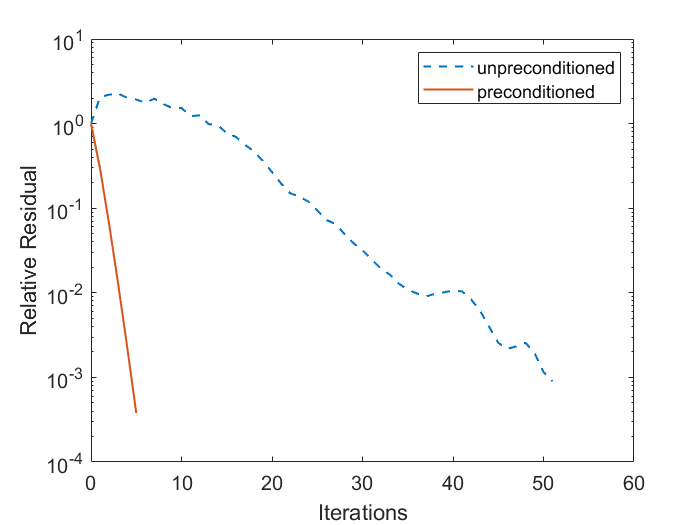
\includegraphics[height=6cm]{2_7_1.png}
    \caption{relative residual of CG and PCG }
  \end{figure}

  In Figure 1.1 the solid line is a plot of $\|r_k\|_2/\|b\|_2$
  for the preconditioned iteration and the dashed line for the
  unpreconditioned. Note that the unpreconditioned reduction in
  $\|r\|$ is not monotone. This is consistent  
  with the theory, which predicts decrese in $\|e\|_A$ but not
  necessarily in $\|r\|$ as the iteration progresses.
  
  \begin{figure}[H]
    \centering\label{fig:2.7.2}
    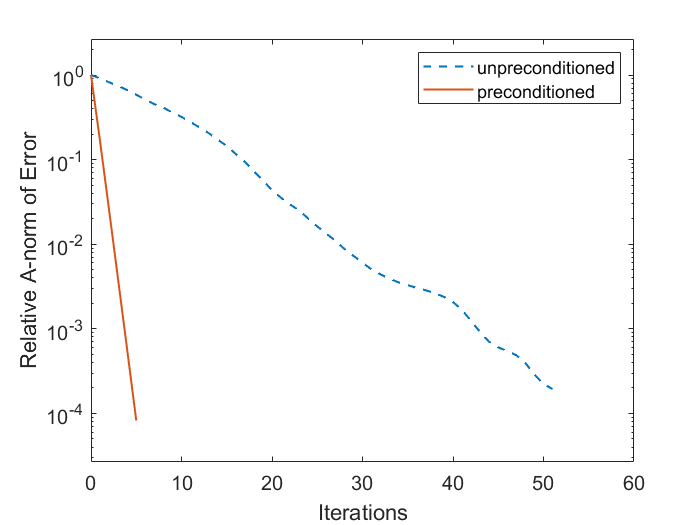
\includegraphics[height=6cm]{2_7_2.png}
    \caption{relative error of CG and PCG }
  \end{figure}
  
   In Figure 1.2 the solid line is a plot of $\|u^*-u_k\|_A/\|u^*-u_0\|_A$
  for the preconditioned iteration and the dashed line for the
  unpreconditioned.  The preconditioned iteration required 5
  iterations for convergence and the unpreconditioned iteration
  52. Note that the unpreconditioned iteration is slowly 
  convergent. This can be explained by the fact that the eigenvalues
  are not clustered and $$\kappa(A)=O(1/h^2)=O(n^2)=O(N).$$
\end{exm}

\subsection{CGNR and CGNE}
\label{sec:2.6}

\begin{defi}
  If $A$ is nonsingular and nonsymmetric, one might consider solving
  $Ax=b$ by applying CG to the normal equations
  \begin{equation}
    \label{eq:2.32}
    A^TAx=A^Tb.
  \end{equation}
  This approach is called CGNR.
\end{defi}

\begin{rmk}
  The reason for this name is that the minimization property of CG as
  applied to \eqref{eq:2.32} asserts that
  \begin{equation*}
    \begin{aligned}
      \|x^*-x\|^2_{A^TA}&=(x^*-x)^TA^TA(x^*-x) \\
      &=(Ax^*-Ax)^T(Ax^*-Ax)=\|r\|^2_2
    \end{aligned}
  \end{equation*}
  is minimized over $x_0+\mathcal{K}_k$ at each iterate. Hence it is
  called CG on the Normal equations to minimize the Residual.
\end{rmk}

\begin{defi}
  If $A$ is nonsingular and nonsymmetric, one could also consider
  applying CG to the normal equations
  \begin{equation}
    \label{eq:2.32}
    AA^Ty=b
  \end{equation}
  and then set $x=A^Ty$. This approach is called CGNE.
\end{defi}

\begin{rmk}
  The reason for this name is that the minimization property of CG as
  applied to \eqref{eq:2.32} asserts that
  \begin{equation*}
    \begin{aligned}
      \|y^*-y\|^2_{AA^T}&=(y^*-y)^TAA^T(y^*-y) \\
      &=(A^Ty^*-A^Ty)^T(A^Ty^*-A^Ty)\\&=\|x^*-x\|_2^2
    \end{aligned}
  \end{equation*}
  is minimized over $y_0+\mathcal{K}_k$ at each iterate. Hence it is
  called CG on the Normal equations to minimize the Error.
\end{rmk}

\begin{rmk}
  There are three  disadvantages that may or may not be serious:
  \begin{itemize}
  \item The condition number of $A^TA$ is the square of that of $A$.
  \item Two matrix-vector products are needed for each CG iterate
    since $\omega=A^T(Ap)$ in CGNR and $\omega=A(A^Tp)$ in CGNE.
  \item One must compute the action of $A^T$ on a vector as part of
    the matrix-vector product involving $A^TA$.
  \end{itemize}
\end{rmk}

%%% Local Variables:
%%% mode: latex
%%% TeX-master: "GMRES_MathDocument"
%%% End:
